\chapter{Első lépések a Calckal}
\thispagestyle{empty}

\section{Adatok bevitele és módosítása}

A Calc program elindítása után az A1 cella az aktív. A
billentyűzeten begépelt karakterek ebbe a cellába kerülnek. A
beírt adatot az Enterrel vagy az iránybillentyűkkel
nyugtázhatjuk. A cella tartalmát módosíthatjuk az F2
funkcióbillentyűvel, vagy kettős kattintással az adott
cellán. 

\begin{figure}[!h]
\begin{center}
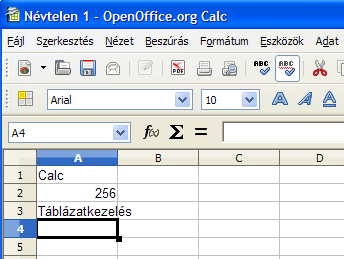
\includegraphics[width=8.102cm]{oocalcv1-img5.png}
\caption{Adatok bevitele}\label{Adatbevitel}
\end{center}
\end{figure}

\Aref{Adatbevitel} ábrán látjuk, hogy szám beírása esetén a Calc
automatikusan jobbra igazítja a tartalmat,  szöveg esetén
viszont balra. Amennyiben a beírt szöveg nem fér el a cellában,
és a tőle jobbra lévő cella üres, a cella tartalma
átcsúszik ebbe a cellába.

Adatot írva a cellába, esetünkben a B3-ba, az A3-as tartalmának
csak egy részét látjuk és a Calc erre a cella jobb szélén
megjelenő nyíllal figyelmeztet (\ref{AdatcellaTúl} ábra).

\begin{figure}[!h]
\begin{center}
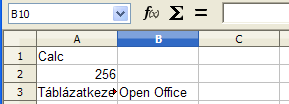
\includegraphics[width=7.645cm]{oocalcv1-img6.png}
\caption{Adatcella határán túlérő tartalom}\label{AdatcellaTúl}
\end{center}
\end{figure}

Az A oszlop szélességét módosíthatjuk, ha az
egér-mutatóját az A és a B oszlopazonosító elválasztó
vonalára vezetjük és bal gombját lenyomva tartva elmozdítjuk
az egeret. Ilyenkor a leendő oszlopszélességet a Calc
megjeleníti cm-ben (\ref{Oszlopszélesség} ábra). Az oszlopazonosítók
 elválasztó vonalára kettőt kattintva a Calc automatikusan a
legtöbb karaktert tartalmazó cellához igazítja az
oszlopszélességet.

\begin{figure}[!h]
\begin{center}
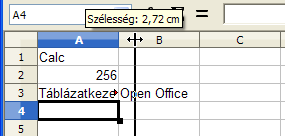
\includegraphics[width=7.539cm]{oocalcv1-img7.png}
\caption{Oszlopszélesség}\label{Oszlopszélesség}
\end{center}
\end{figure}

Számadattal nem fordulhat elő, hogy csak egy részét látjuk a
cellában. Amennyiben a számjegyek nem férnek el, a Calc mindig
kettős keresztekkel figyelmeztet erre (\ref{KeskenyOszlop}).

\begin{figure}[!h]
\begin{center}
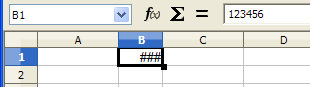
\includegraphics[width=8.2cm]{oocalcv1-img8.png}
\caption{Kicsi oszlopszélesség \#\#\#}\label{KeskenyOszlop}
\end{center}
\end{figure}

Többsoros szöveget is írhatunk a cellába, amennyiben a
Ctrl+Enter billentyűkkel zárjuk a sort. Hatására
lehetőség nyílik az új sor kezdéséhez. Ilyenkor a Calc
automatikusan megnöveli a sormagasságot.


\section{Kijelölés}

Az aktív cellán különböző formázásokat,
beállításokat végezhetünk. Több cella formátumának
 módosításához kijelöléssel meghatározhatunk cellákat,
téglalap alakú cellatartományokat. A Calc-ban egyszerűen
kijelölhetünk cellatartományokat: a tartomány egyik
sarokcellájára kattintva, az egér bal gombját lenyomva tartva
átlósan húzva. Egy ilyen tartományt bal felső és a jobb
alsó cellák címeivel, és közöttük kettősponttal
határozunk meg. Pl. A1:B5.

Billentyűzet segítségével, a SHIFT billentyűt lenyomva
tartva az iránybillentyűkkel jelölhetünk ki.

Több különálló cellát vagy cellatartományt is
kijelölhetünk. Ehhez az első kijelölése után a többit,
a Ctrl billentyűt lenyomva tartva kell kijelölnünk.

Egy oszlop vagy sor minden celláját kijelölhetjük az oszlop-,
illetve a sorazonosítóra kattintva. A munkalap bal felső
sarkában lévő üres téglalapra kattintva a munkalap minden
celláját kijelöljük (\ref{MunkalapKijelölés} ábra)

\begin{figure}[!h]
\begin{center}
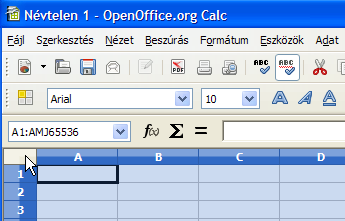
\includegraphics[width=9.126cm]{oocalcv1-img9.png}
\caption{Munkalap kijelölése}\label{MunkalapKijelölés}
\end{center}
\end{figure}

Két vagy több kijelölt cellát egyesíthetünk egy cellába a
\textbf{Formázás} eszköztár \textbf{Cellák egyesítése}
parancsával. Az így kialakult terület elfoglalja a kijelölt
cellákat, és erre a tartományra a bal cella címével
hivatkozhatunk. \Aref{CellákEgyesítése} ábrán az A3:C3 tartományt
egyesítettük egy cellává. Ennek a cellacíme A3. 

\begin{figure}[!h]
\begin{center}
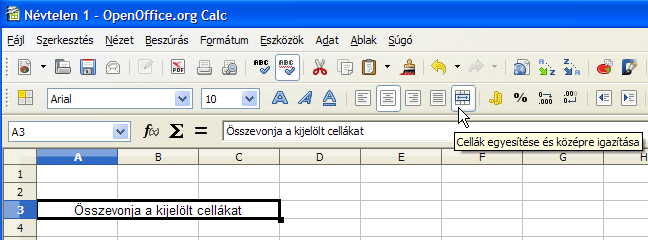
\includegraphics[width=15.999cm]{oocalcv1-img10.png}
\caption{Cellák összevonása}\label{CellákEgyesítése}
\end{center}
\end{figure}


\section{Cellák formázása}

A gyakran használt cellákra vonatkozó formátumokat
legegyszerűbben a \textbf{Formátum} eszköztáron érhetjük
el. A \textbf{Calc} képes a karakterek beírása közben
módosítani a formátumot. \Aref{CellákFormázása} ábrán látható
karakterformátumok a szöveg begépelése közben a
\textbf{Formátum} eszköztár parancsaival lettek kialakítva.

\begin{figure}[!h]
\begin{center}
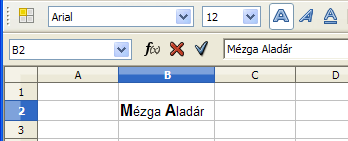
\includegraphics[width=9.206cm]{oocalcv1-img11.png}
\caption{Cellák formázása}\label{CellákFormázása}
\end{center}
\end{figure}

További, az eszköztáron nem elérhető formátumokat a
\textbf{Formátum} menü \textbf{Cellák...}, vagy a helyi menü
\textbf{Cellák formázása} paranccsal állíthatunk be. A
megjelenő párbeszédablakban a \textbf{Betűkészlet} és a
\textbf{Betűhatások} füleken a cellára vonatkozó
karakterformátumokat módosíthatjuk. 

Az \textbf{Igazítás} fülön (\ref{CellákIgazítása} ábra) beállíthatjuk az
aktuális vagy a kijelölt cellák tartalmának igazítását. A
vízszintes szövegigazítások közül az
\textbf{Alapértelmezett} a számokat jobbra, a szöveget balra
igazítja. A következő négy (balra, jobbra, középre és
sorkizárt) elérhető a Formázás eszköztáron is. A
\textbf{Kitöltött} szövegigazítás megismétli a
cellatartalmakat (számokat és szövegeket), amíg a cella
látható területét ki nem tölti.

\begin{figure}[!h]
\begin{center}
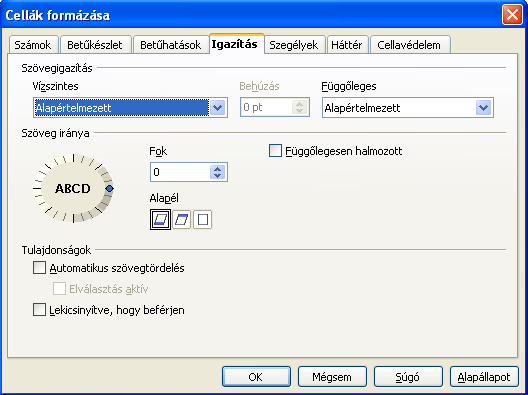
\includegraphics[width=12.97cm]{oocalcv1-img12.png}
\caption{Cellák formázása --  Igazítás}\label{CellákIgazítása}
\end{center}
\end{figure}

A \textbf{Szöveg iránya} részben megadhatjuk a kijelölt cellák
elforgatásának szögét fokokban, de megadhatjuk a
szövegirányt az ABCD feliratú körlapra kattintva is.

Figyeljük meg \aref{Cellaformátumok} ábrán látható cellaformátumokat.
A C2 cellában a vízszintes és a függőleges szövegigazítás
beállítása: \textbf{Középre.} Az \textbf{Automatikus
szövegtördelés} és az \textbf{Elválasztás} is be van
kapcsolva.

A D2 cella mind függőlegesen, mind vízszintesen középre
igazított, és a \textbf{Függőlegesen halmozott} formátum is
be van kapcsolva. 

A C1 cella balra igazított, a behúzás mértéke 10 pt.

\begin{figure}[!h]
\begin{center}
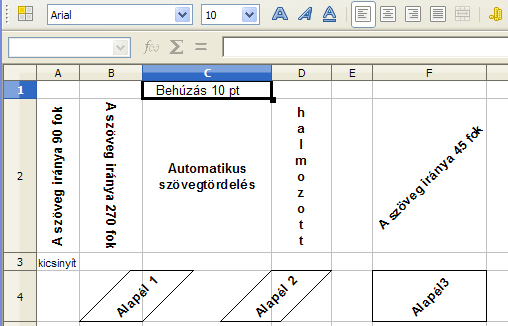
\includegraphics[width=12.439cm]{oocalcv1-img13.png}
\caption{Cellaformátumok}\label{Cellaformátumok}
\end{center}
\end{figure}

Az A3 cella betűmérete és formátuma nem különbözik a C1
celláénál, de a \textbf{Lekicsinyítve, }\textbf{hogy
beférjen} kapcsoló be van kapcsolva.

A B4, D4 és az F4 szegéllyel ellátott cellákon az Alapél
három beállítását figyelhetjük meg. Mindhárom cellában
a szöveg iránya 45 fokkal el van forgatva. A B4 cellában az
elforgatott szöveg a cella alsó szélétől kifelé jelenik
meg. A D4 esetében a felső szélétől kifelé, az F4-ben
pedig az elforgatott szöveg csak a cellába kerül.


\section{Karakterformázás}

A cella tartalmának módosításakor a kijelölt karakteren
különleges formázásokat is végrehajthatunk. Ezek
elérhetőek a \textbf{Formátum} menü \textbf{Karakter}
párbeszédablakban a  \textbf{Betűkészlet},
\textbf{Betűhatások} és \textbf{Betűhelyzet} fülekre
kattintva. Gyorsmenü segítségével szintén elérhetők
ezek a beállítások, ha a kijelölt szövegrészen az egér
jobb gombjával kattintunk (\ref{KarakterStílus} ábra).

\begin{figure}[!h]
\begin{center}
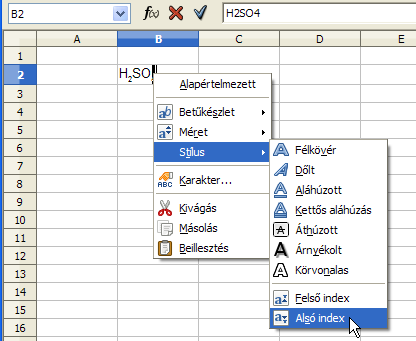
\includegraphics[width=10.005cm]{oocalcv1-img14.png}
\caption{Karakterformázás --  Stílus}\label{KarakterStílus}
\end{center}
\end{figure}

\section{Szegélyek és háttér}

A Calc alapbeállítása szerint a képernyőn látható
szürke színű rácsvonalak nyomtatásban nem jelennek meg.
Nyomtatásban is látható rácsvonalakat legegyszerűbben a
Formátum eszköztár \textbf{Szegélyek} ikonjára kattintva
hozhatunk létre (\ref{SzegélyekIkon} ábra).  Ilyenkor az aktív
cella, vagy a kijelölt cellatartomány az általunk választott
szegélytípust kapja.

\begin{figure}[!h]
\begin{center}
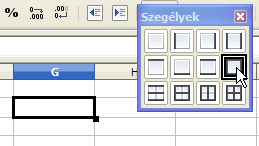
\includegraphics[width=7.351cm]{oocalcv1-img15.png}
\caption{Szegélyek ikon, menü}\label{SzegélyekIkon}
\end{center}
\end{figure}

Egyéni szegélybeállításokat a \textbf{Formátum} menü
\textbf{Cellák} parancsát választva, a párbeszédablak
\textbf{Szegélyek} lapján állíthatunk be (\ref{CellaSzegélyek} ábra).
Választhatunk vonalvastagságot, stílust, színt és akár
árnyékolást is. A \textbf{Szegély elrendezése} terület
másképp jelenik meg attól függően, hogy cellát,
cellákat egy oszlopban, cellákat egy sorban vagy nagyobb
cellatartományt jelölünk ki. Ezek a lehetőségek a
cellatartományok belső, átlós és cellákon belüli
átlós szegélyeire vonatkoznak.

\begin{figure}[!h]
\begin{center}
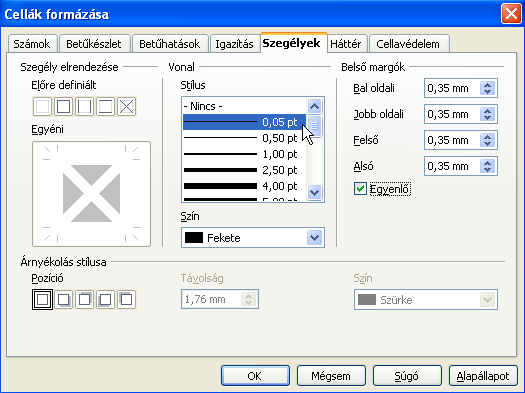
\includegraphics[width=13.891cm]{oocalcv1-img16.png}
\caption{Cellák formázása --  Szegélyek}\label{CellaSzegélyek}
\end{center}
\end{figure}

Az \textbf{Egyéni} területen kattintásokkal állíthatunk be
vonalakat. Ezek jelentése a következő:
\begin{description}
\item [Fekete vonal] -- beállítja a kijelölt cellákra a
kiválasztott stílusú vonalat. Szaggatott vonal akkor jelenik meg,
ha 0,05 pontos vonalstílus van kiválasztva.
\item [Szürke vonal] -- a kijelölt cellák megfelelő vonala
nem fog változni
\item [Fehér vonal] -- a kijelölt cellák megfelelő vonalai
törölve lesznek. 
\end{description}

Az aktív cella, vagy a kijelölt cellatartomány
háttérszínét a \textbf{Formátum} menü \textbf{Cellák}
parancsát választva, a párbeszédablak \textbf{Szegélyek}
lapján állíthatjuk be. 


\section{Munkafüzet mentése}

Munkafüzetünket a \textbf{Fájl} menü vagy a \textbf{Standard}
eszköztár \textbf{Mentés} parancsával menthetjük el. A Calc
alapértelmezett formátuma az OpenDocument, amely az irodai
dokumentumok új, nemzetközi szabványa. Az OpenDocument
munkafüzet állományának kiterjesztése .ods. A Calc képes
Microsoft Excel formátumba is menteni munkafüzetünket, amennyiben
a Fájl típusánál ezt választjuk (\ref{FájlFormátumok} ábra).

\begin{figure}[!h]
\begin{center}
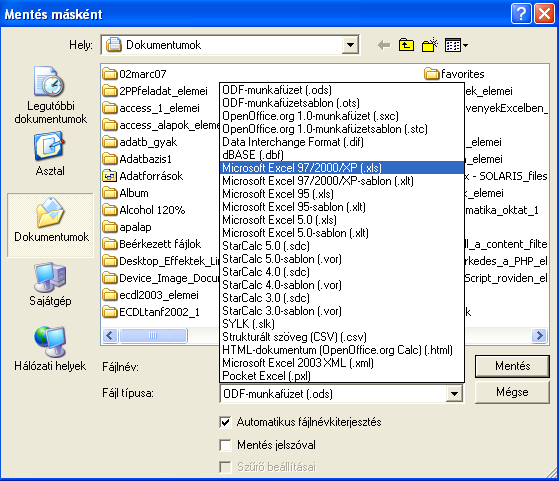
\includegraphics[width=13.79cm]{oocalcv1-img17.png}
\caption{Fájl mentése --  fájlformátumok}\label{FájlFormátumok} 
\end{center}
\end{figure}

A \textbf{Mentés} ablak, attól függően, hogy milyen
operációs rendszeren használjuk a Calcot, formailag
különbözhet. \Aref{FájlFormátumok} ábrán a Microsoft Windows XP-re
telepített Calc \textbf{Mentés} ablakát látjuk.

Az alapértelmezett mentési formátum és mentési hely
módosítható az \textbf{Eszközök} menüpont
\textbf{Beállítások} parancs kiadásakor megjelenő
párbeszédablakban (\ref{MegnyitásMentés} ábra).
A mentési helyet az \textbf{OpenOffice.org} --
\textbf{Útvonalak} --  \textbf{Dokumentumok} lehetőséget
választva módosíthatjuk. Az alapértelmezett  fájlformátum
 a \textbf{Megnyitás és mentés} -- \textbf{Általános}
ablakban állítható be, a dokumentum típusánál a
munkafüzetet választva.

\begin{figure}[!h]
\begin{center}
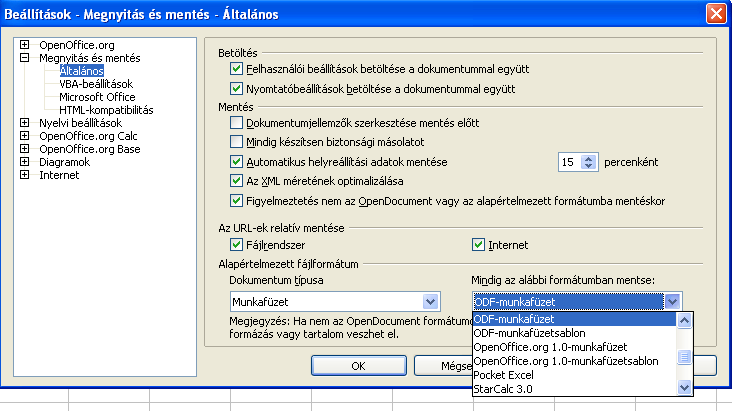
\includegraphics[width=14.999cm]{oocalcv1-img18.png}
\caption{Általános beállítások --  Megnyitás és mentés}\label{MegnyitásMentés}
\end{center}
\end{figure}


\section{1. feladat}

{\itshape
Hozzuk létre a képen látható táblázatot (\ref{1-feladat} ábra) és
mentsük el a munkafüzetet \textbf{calc01} néven OpenDocument
formátumban!}

A munkalap neve legyen ZH 01. Az egyesített B1:G1 tartományban
Ctrl+Enter segítségével hozzunk létre sortörést. A C4:G4
cellatartomány függőleges szegélyvonalai fehér
színűek.

\begin{figure}[!h]
\begin{center}
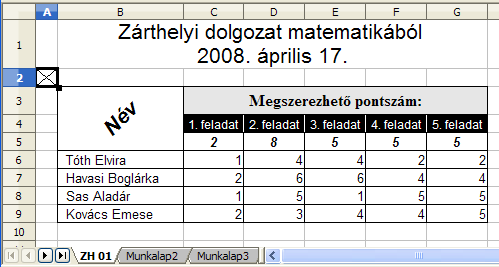
\includegraphics[width=10.673cm]{oocalcv1-img19.png}
\caption{1. feladat}\label{1-feladat}
\end{center}
\end{figure}

